\documentclass{../../submodules/TEX/document/ug/ug}
\usepackage{float}
\usepackage{color, colortbl}
\usepackage[section]{placeins}
\usepackage{mathtools}
\usepackage{amsthm}
%\usepackage[T1]{helvet}
\usepackage[OT1]{fontenc} 


\theoremstyle{plain}
\newtheorem*{defn*}{Definition}
\newtheorem*{ex*}{Example}


\title{IObundle Example User Guide}
\category{User Guide}

%\getenv[\TEX]{TEX_DIR}
\definecolor{iob-green}{rgb}{0.0,1.0,0.80}
\definecolor{iob-blue}{rgb}{0.90196,0.94902,1}


\begin{document}
\maketitle
\cleardoublepage
\tableofcontents
\clearpage
\listoftables
\clearpage
\listoffigures
\cleardoublepage

\section{\textcolor[rgb]{0,0,0}{Introduction}}
\lipsum[1-1]


\section{Symbol}
\begin{figure}[!htbp]
    \centerline{\includegraphics[width=14cm]{symb.png}}
    \vspace{0cm}\caption{IP Core Symbol}
    \label{fig:i2score_sym}
\end{figure}



\section{\textcolor[rgb]{0,0,0}{Features}}
\begin{itemize}
\item f1
\item f2
\end{itemize}


\section{\textcolor[rgb]{0,0,0}{Benefits}}
\begin{itemize}
\item Easy hardware and software integration
\item Compact hardware implementation
\item Can fit many instances in low cost FPGAs
\item Can fit many instances in small ASICs 
\item Low power consumption
\end{itemize}


\section{\textcolor[rgb]{0,0,0}{Deliverables}}
\begin{itemize}
\item ASIC or FPGA synthesized netlist or Verilog source code
\item Verification environment with testbench
\item User documentation for easy system integration
\item Example integration in IOb-SoC (optional)
\item ASIC or FPGA synthesis and implementation scripts or
\end{itemize}


\section*{\textcolor[rgb]{0,0,0}{Block Diagram}}
\begin{figure}[H]
  \vspace{-.5cm}
  \centering {\includegraphics[width=\columnwidth]{bd.pdf}}
  \vspace{-0.7cm}
  \caption{High-level block diagram}
  \label{fig:bd}
\end{figure}


\section{Interface Signals}

\begin{table}[H]
  \begin{center}
    \begin{tabular}{|l|l|p{8cm}|}
      \hline
      \rowcolor{iob-green}
      \textbf{Signal} & \textbf{Direction} & \textbf{Description} \\
      \hline
      \hline

     % \input is_tab.tex

    \end{tabular}
    \caption{General interface signals}
    \label{tab:is}
  \end{center}
\end{table}


\section{Timing Diagrams}

\begin{figure}[H]
  \begin{center}
    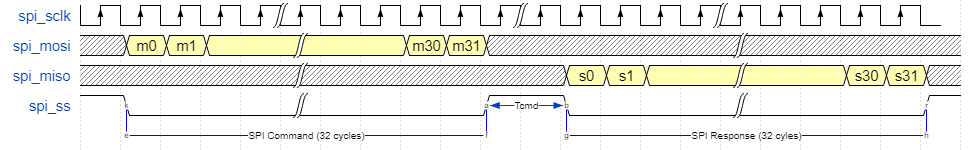
\includegraphics[width=16cm]{spi.png}
    \caption{SPI slave interface timing diagram}
    \label{fig:spi}
  \end{center}
\end{figure}

\section{Software Components}

\section*{FPGA Resources}
\begin{table}[H]
\ifnum\XILINX=1
\ifnum\INTEL=1
\begin{minipage}{0.45\linewidth}
\else
\begin{minipage}{\linewidth}
\fi
\centering
\begin{tabular}{|l|r|}
\hline
\rowcolor{iob-green}
\textbf{Resource}  & \textbf{Used} \\
\hline
\hline
\input xil_results.tex 
\end{tabular}
\end{minipage}
\fi
\ifnum\INTEL=1
\ifnum\XILINX=1
\begin{minipage}{0.45\linewidth}
\else
\begin{minipage}{\linewidth}
\fi
\centering
\begin{tabular}{|l|r|}
\hline
\rowcolor{iob-green}
\textbf{Resource}  & \textbf{Used} \\
\hline
\hline
\input alt_results.tex 
\end{tabular}
\end{minipage}
\fi
\ifnum\INTEL=1
\ifnum\XILINX=1
\caption{FPGA results for Kintex Ultrascale (left) and Cyclone V GT (right)}
\fi
\ifnum\XILINX=0
\caption{FPGA results for Cyclone V GT}
\fi
\fi
\ifnum\XILINX=1
\ifnum\INTEL=0
\caption{FPGA results for Kintex Ultrascale}
\fi
\fi
\end{table}



%\bibliographystyle{unsrt}
%\bibliography{rep}
%\nocite{*}

\end{document}
